\documentclass[11pt,a4paper]{article}
\usepackage[margin=22mm]{geometry}
\usepackage{fontspec}
\setmainfont{texgyretermes}[Extension=.otf,UprightFont=*-regular,BoldFont=*-bold,ItalicFont=*-italic,BoldItalicFont=*-bolditalic]
\setsansfont{texgyreheros}[Extension=.otf,UprightFont=*-regular,BoldFont=*-bold]
\setmonofont{lmmono10-regular.otf}
\usepackage{microtype,booktabs,array,tabularx,graphicx,amsmath}
\usepackage[font=small,labelfont=bf]{caption}
\usepackage{float,needspace,titlesec,fancyvrb,placeins}
\usepackage[hidelinks,unicode]{hyperref}
\urlstyle{same}
\setlength{\parindent}{0pt}
\setlength{\parskip}{3pt plus 1pt}
\setlength{\textfloatsep}{10pt}
\setlength{\intextsep}{9pt}
\renewcommand{\arraystretch}{1.13}
\titleformat{\section}{\large\bfseries}{\thesection.}{0.5em}{}
\titleformat{\subsection}{\normalsize\bfseries}{\thesubsection}{0.5em}{}
\titlespacing*{\section}{0pt}{10pt}{5pt}
\titlespacing*{\subsection}{0pt}{7pt}{3pt}
\clubpenalty=10000 \widowpenalty=10000
\emergencystretch=1em
\DeclareCaptionType{listing}[Listing][List of Listings]
\begin{document}

{\centering\LARGE\bfseries Reproducing A-MEM: A Cost-Aware Study of Memory Linking and Evolution\par}
\vspace{5pt}{\centering\small FTEC5660 — Agentic AI for Business and FinTech  |  Individual Reproducibility Assignment\par}
{\centering\small Paper: Xu et al. (2025), A-MEM: Agentic Memory for LLM Agents  |  Code and evidence: \href{https://github.com/alistairkung/A-mem-reproducibility}{github.com/alistairkung/A-mem-reproducibility}\par}\vspace{8pt}
\noindent{\small Student name: Alistair Chi Chuen Kung \hfill Student ID: 1155012046}\par
\section{Project summary and research questions}
Xu et al. report that answer scores rise from Neither to Linking Only to Full A-MEM on both metrics in all five question categories~\cite{xu2025amem}. I set out to reproduce that pattern and to measure the contribution of each memory action. The published comparison leaves one case open: updating older memories when linking is disabled. I also wanted to know how changes in answer quality compared with the model charges for each configuration.

\textbf{Part A. Reproducing the advantage.} The Full implementation reproduced the frozen author workflow exactly in replay. On three preselected LoCoMo conversations, Full repeated the published category win on both metrics in three of five categories. Only adversarial questions repeated the entire three-way ordering. In my supplementary analysis of 558 questions, the same saved answers put Full first under historical F1 (32.69\%) and Neither first under updated author F1 (39.00\%).

\textbf{Part B. Attributing the advantage.} I added Evolution Only to test whether neighbour updates help temporal reasoning independently. On 89 temporal questions, enabling updates changed F1 by $-2.44$ percentage points without linking and $+2.67$ with it. Neither still had the highest temporal F1. Across all questions, Evolution Only scored below Neither under both scoring conventions and cost slightly more.

\subsection{Cost-aware scope}
The released LoCoMo sample~\cite{locomo} contains ten conversations, 5,882 turns and 1,986 questions. Running all four configurations would require forty builds, each processing a conversation turn by turn. The coursework brief allowed a smaller, clearly defined experiment. I kept all four configurations and reduced the number of conversations, selecting three by length stratum with a fixed seed (42) before inspecting scores. This gave twelve independent builds, one per cell, and the same 558 questions for every configuration.

\begin{table}[H]\centering\small\setlength{\tabcolsep}{4pt}
\begin{tabular}{@{}>{\raggedright\arraybackslash}p{\dimexpr 0.48\linewidth-5.333333333333333pt\relax}>{\raggedright\arraybackslash}p{\dimexpr 0.25\linewidth-5.333333333333333pt\relax}>{\raggedright\arraybackslash}p{\dimexpr 0.27\linewidth-5.333333333333333pt\relax}@{}}
\toprule
Conversation & Turns & Questions \\
\midrule
conv-44 & 675 & 158 \\
conv-49 & 509 & 196 \\
conv-50 & 568 & 204 \\
Total per condition & 1,752 & 558 \\
\bottomrule\end{tabular}
\caption{Preselected LoCoMo evaluation population (558 questions per configuration).}\label{tab1}
\end{table}
\section{A-MEM and experimental setup}
\subsection{Memory construction and retrieval}
For each conversational turn, an LLM stores the original content with generated keywords, context and tags. MiniLM embeddings identify up to five nearby memories. A shared LLM decision proposes two actions. \emph{Strengthen} adds outgoing links and may revise tags on the new note. \emph{Update neighbour} can change contexts and tags on older notes while preserving their original content. After insertion, the note is available for answering questions. Answer retrieval starts with ten similar notes and can follow links to additional entries.

Neither still creates notes and metadata, retrieves memories and requests the shared decision whenever the frozen routine calls for it. The four configurations vary which proposed actions may change memory. All incur the cost of generating shared decisions.

\subsection{Frozen runtime and reproducibility}
The frozen author implementation~\cite{amemsource} was fixed to commit \href{https://github.com/WujiangXu/A-mem/commit/f9a173dec325d84fcc97e7828775c7b241c33466}{f9a173d}. The accepted GPT-4o-mini campaign used openai/gpt-4o-mini-2024-07-18 via OpenRouter, with OpenAI pinned as the upstream provider. Each cell used separate memory, retrieval-index and response-cache state. Prompts and native output contracts were fixed; temperature was 0.7 except for category-5 answers at 0.5. Construction neighbours were k=5; answer retrieval began at k=10. A 4,096-token limit applied to evolution decisions and 1,000 tokens to other stages. The recorded Python environment used Python 3.11.17 for publication reproducibility.

Deterministic replay used the archived DeepSeek responses from conv-50. The gated Full routine matched the frozen author routine at 568 memory insertion states, 1,544 requests and 204 answers. Separate tests verified that disabled actions left prohibited fields untouched and that per-condition memory stores stayed independent (Section~4). For the GPT-4o-mini comparison, each configuration built fresh memories~\cite{reproduction,acceptedresults}.

\section{Reproduction target and evaluation}
\subsection{The published comparison}
Table~3 of Xu et al. reports F1 and BLEU-1 for each question category~\cite{xu2025amem}. Within every category both scores rise from Neither to Linking Only to Full. I reconstructed Neither and Linking Only alongside Full on our three selected conversations and compared category scores under historical evaluation (Section~5.1). I then assessed how the authors’ updated reference changed our own question-weighted comparison (Section~5.2).

\subsection{What the metrics mean}
The released F1 scorer treats words as sets. Precision measures the share of distinct predicted words that appear in the reference, recall the share of reference words recovered. F1 is their harmonic mean. BLEU-1 measures unigram overlap and penalises short predictions. A valid paraphrase can score poorly on either metric. I score each question and take equal-weight means over the stated population.

\subsection{What the five question categories test}
\begin{table}[H]\centering\small\setlength{\tabcolsep}{4pt}
\begin{tabular}{@{}>{\raggedright\arraybackslash}p{\dimexpr 0.18\linewidth-5.333333333333333pt\relax}>{\raggedright\arraybackslash}p{\dimexpr 0.12\linewidth-5.333333333333333pt\relax}>{\raggedright\arraybackslash}p{\dimexpr 0.7\linewidth-5.333333333333333pt\relax}@{}}
\toprule
Category & Questions & What the question requires \\
\midrule
Multi-hop & 99 & Combine facts scattered across multiple conversation turns. \\
Temporal & 89 & Reason about dates, sequences and changes over time. \\
Open-domain & 27 & Apply general knowledge or contextual understanding to conversation evidence. \\
Single-hop & 222 & Retrieve a directly stated conversational fact. \\
Adversarial & 121 & Recognise when the conversation does not supply the requested information. \\
\bottomrule\end{tabular}
\caption{The five LoCoMo question categories in the selected 558-question population.}\label{tab2}
\end{table}
\subsection{Historical and updated author evaluation}
The \href{https://github.com/WujiangXu/A-mem/commit/236670fefd1407ac63bcae29dd0de7fb206f569a}{historical evaluator} used the supplied distractor as the Category~5 reference. On 22 October 2026, before the study protocol was frozen, the authors changed the default to “Not mentioned in the conversation” and kept \verb|--legacy_c5_reference| for historical scoring~\cite{xu2026scoring}. Our initial specification (\href{https://github.com/alistairkung/A-mem-reproducibility/commit/5aaa5f693b7315bf2e668d7540cebbe7523f96b7}{D11}) designated updated author evaluation as primary and historical evaluation as secondary for the paper comparison.

Our \href{https://github.com/alistairkung/A-mem-reproducibility/commit/60e109ef4de25db97f3f0fea6bd65fffc276515c}{T4 implementation} applies the same author F1 and BLEU-1 functions to each saved prediction twice. Only the reference for the 121 adversarial questions changes. A separate binary score records whether the model identified missing information. That count stays fixed when the overlap reference changes.

\begin{table}[H]\centering\small
\begin{tabular}{@{}lrr@{}}
\toprule
Saved response & Historical F1 / BLEU-1 & Updated F1 / BLEU-1 \\
\midrule
Audrey (Full A-MEM), abstained & 18.18 / 16.37 & 100 / 100 \\
Dave (Evolution Only), chose distractor & 100 / 100 & 0 / 0 \\
\bottomrule\end{tabular}
\caption{Two verified Category 5 predictions from the accepted GPT-4o-mini experiment. Each row scores one saved answer under both references (percent).}\label{tab3}
\end{table}
Audrey described a pet-bonding workshop. Asked why she had signed up for a car maintenance workshop, Full A-MEM answered “Not mentioned in the conversation”. Only the word “the” overlaps the historical reference “Strengthen the bond with her pets”. Dave described restoring old cars. Asked what he found satisfying about destroying them, Evolution Only gave the distractor verbatim: “Transforming something old and beat-up into something beautiful”. The binary abstention scores are 1 for Audrey’s question and 0 for Dave’s under either view. The \href{https://github.com/alistairkung/A-mem-reproducibility/blob/930254d9c4c1c430899a25fe42a94fa164a85812/reports/adversarial_scoring_audit/five_examples.md}{five-example audit} gives the derivations for conv-44:qa:126 and conv-50:qa:183, respectively.

\section{Modification, experimental wrapper and verification}
\subsection{Completing the factorial design}
\begin{table}[H]\centering\small\setlength{\tabcolsep}{4pt}
\begin{tabular}{@{}>{\raggedright\arraybackslash}p{\dimexpr 0.36\linewidth-5.333333333333333pt\relax}>{\raggedright\arraybackslash}p{\dimexpr 0.3\linewidth-5.333333333333333pt\relax}>{\raggedright\arraybackslash}p{\dimexpr 0.34\linewidth-5.333333333333333pt\relax}@{}}
\toprule
Condition & Strengthen new note & Update existing neighbours \\
\midrule
Neither & OFF & OFF \\
Linking Only & ON & OFF \\
Evolution Only (added) & OFF & ON \\
Full A-MEM & ON & ON \\
\bottomrule\end{tabular}
\caption{Two independently gated action bundles. The shared LLM evolution decision remains in all four conditions.}\label{tab4}
\end{table}
Evolution Only completes the $2\times2$ design. I expected that updating older notes might help with dates, sequences and changes over time. This motivated the temporal comparison, although I did not preregister a temporal endpoint. Linking might also help multi-hop questions that draw on facts from different turns.

\subsection{Wrapper implementation and validation}
The evaluator exposed no switches for the two existing actions. I added a Boolean guard to each branch in the frozen method’s abstract syntax tree (Listing~\ref{lst:gates}). Evolution Only permits neighbour updates while preserving the shared LLM decision, insertion, retrieval and consolidation (Figure~\ref{fig1}).

\begin{minipage}{\linewidth}
\VerbatimInput[fontsize=\footnotesize]{listing.py}
\captionof{listing}{Abridged excerpt from \href{https://github.com/alistairkung/A-mem-reproducibility/blob/8485673183d7b8018c841082d075b21158002700/amem_repro/actions.py}{amem\_repro/actions.py}, commit 8485673. The excerpt omits the equality-operator check, validation and compilation.}\label{lst:gates}
\end{minipage}\par\smallskip
\begin{figure}[H]\centering
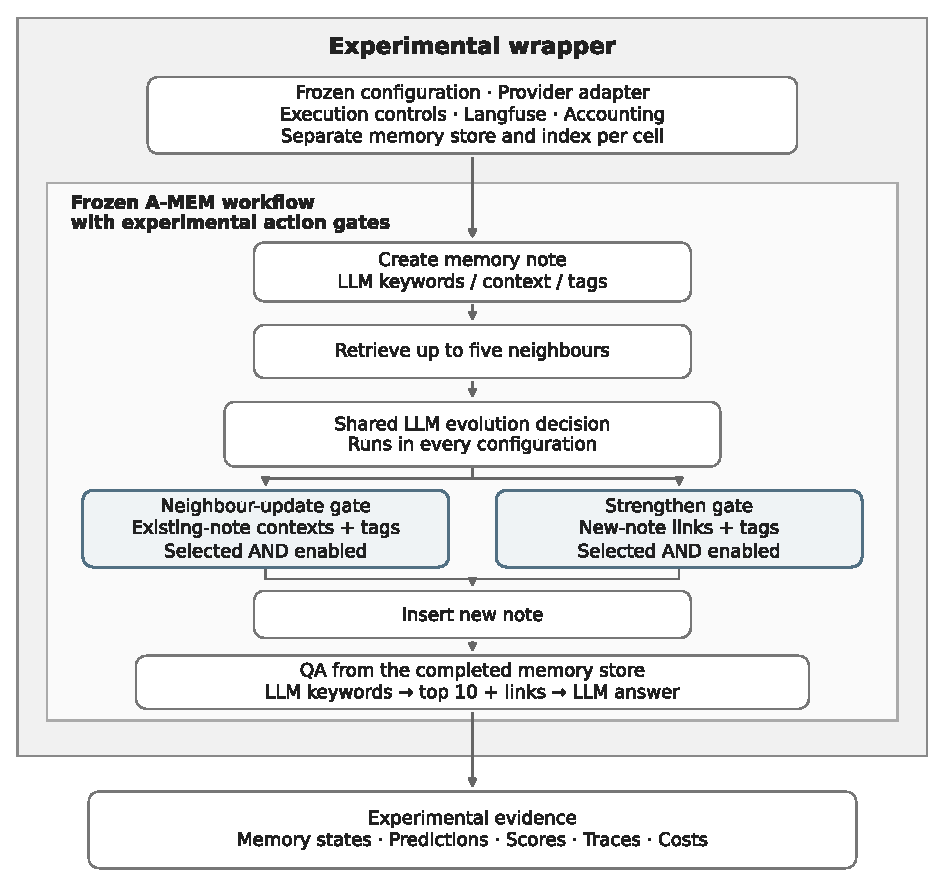
\includegraphics[width=122mm]{assets/amem_wrapper_architecture.pdf}
\captionsetup{hypcap=false}
\caption{The experimental wrapper controls execution, tracing and accounting. The frozen A-MEM workflow supplies the shared decision and applies each selected action when its gate permits it.}\label{fig1}
\end{figure}
Each condition needed its own memory build. The \href{https://github.com/WujiangXu/A-mem/blob/f9a173dec325d84fcc97e7828775c7b241c33466/test_advanced.py#L259-L279}{released evaluator} creates a fresh agent per conversation, but its cache path uses the backend, model, refresh setting and sample index. Reusing that path across conditions could load another condition’s memories. My \href{https://github.com/alistairkung/A-mem-reproducibility/blob/8485673183d7b8018c841082d075b21158002700/amem_repro/runner.py#L233-L263}{runner} includes the condition and enabled actions in the build identity; the \href{https://github.com/alistairkung/A-mem-reproducibility/blob/8485673183d7b8018c841082d075b21158002700/amem_repro/artifacts.py#L80-L96}{cache loader} checks the stored identity before reuse. The published runs’ cache-isolation procedure is unverified.

\subsection{Tracing and financial reconciliation}
Langfuse traced generations, actions, retrieval and scores. For the Pareto comparison I took USD charges from our local journals and ledger. The controller reserved funds before transmission and settled against generation ID, route and native usage. Missing usage kept the full reservation.

\newpage
\section{Results and interpretation}
\subsection{Part A: Which published category results recur?}
Full again won both metrics in open-domain, single-hop and adversarial. Only adversarial retained the complete ordering. On single-hop, Full kept first place and Neither overtook Linking Only for second. Linking Only won multi-hop and Neither won temporal.

\begin{table}[H]\centering\small\setlength{\tabcolsep}{2pt}
\begin{tabular*}{\linewidth}{@{\extracolsep{\fill}}llrrrrr@{}}
\toprule
Configuration & Source & Multi-hop & Temporal & Open-domain & Single-hop & Adversarial \\
\midrule
Neither & Paper & 9.65/7.09 & 24.55/19.48 & 7.77/6.70 & 13.28/10.30 & 15.32/18.02 \\
        & Ours  & 16.86/11.94 & \textbf{36.61/32.80} & 14.37/14.15 & 34.82/28.72 & 30.66/29.90 \\
\addlinespace[2pt]
Linking Only & Paper & 21.35/15.13 & 31.24/27.31 & 10.13/10.85 & 39.17/34.70 & 44.16/45.33 \\
        & Ours  & \textbf{20.25/15.00} & 31.62/28.32 & 12.78/12.86 & 33.75/28.18 & 34.70/34.22 \\
\addlinespace[2pt]
Full A-MEM & Paper & \textbf{27.02/20.09} & \textbf{45.85/36.67} & \textbf{12.14/12.00} & \textbf{44.65/37.06} & \textbf{50.03/49.47} \\
           & Ours & 17.54/11.29 & 34.29/30.13 & \textbf{15.92/16.41} & \textbf{35.94/30.40} & \textbf{41.70/41.24} \\
\bottomrule\end{tabular*}
\caption{Table~3 of Xu et al.~\cite{xu2025amem} and our historical reconstruction~\cite{acceptedresults}. Each pair is F1/BLEU-1 (\%). Bold marks each source’s category winner on both metrics. Our sample sizes are 99, 89, 27, 222 and 121, respectively.}\label{tab:direct}
\end{table}


\subsection{How the reference changes our aggregate ranking}
\begin{table}[H]\centering\small\setlength{\tabcolsep}{4pt}
\begin{tabular}{@{}>{\raggedright\arraybackslash}p{\dimexpr 0.18\linewidth-6.666666666666667pt\relax}>{\raggedright\arraybackslash}p{\dimexpr 0.14\linewidth-6.666666666666667pt\relax}>{\raggedright\arraybackslash}p{\dimexpr 0.16\linewidth-6.666666666666667pt\relax}>{\raggedright\arraybackslash}p{\dimexpr 0.125\linewidth-6.666666666666667pt\relax}>{\raggedright\arraybackslash}p{\dimexpr 0.195\linewidth-6.666666666666667pt\relax}>{\raggedright\arraybackslash}p{\dimexpr 0.20\linewidth-6.666666666666667pt\relax}@{}}
\toprule
Configuration & Historical F1 & Hist. BLEU-1 & Updated F1 & Updated BLEU-1 & Adversarial correct \\
\midrule
Neither & 30.03 & 25.95 & 39.00 & 35.01 & 86/121 \\
Linking Only & 30.21 & 26.43 & 37.34 & 33.57 & 80/121 \\
Evolution Only & 29.29 & 25.69 & 35.86 & 32.29 & 79/121 \\
Full A-MEM & 32.69 & 28.64 & 36.91 & 32.81 & 71/121 \\
\bottomrule\end{tabular}
\caption{Question-weighted percentages on all 558 matched questions per configuration; two reference policies applied to the same saved predictions.}\label{tab5}
\end{table}
\begin{figure}[H]\centering
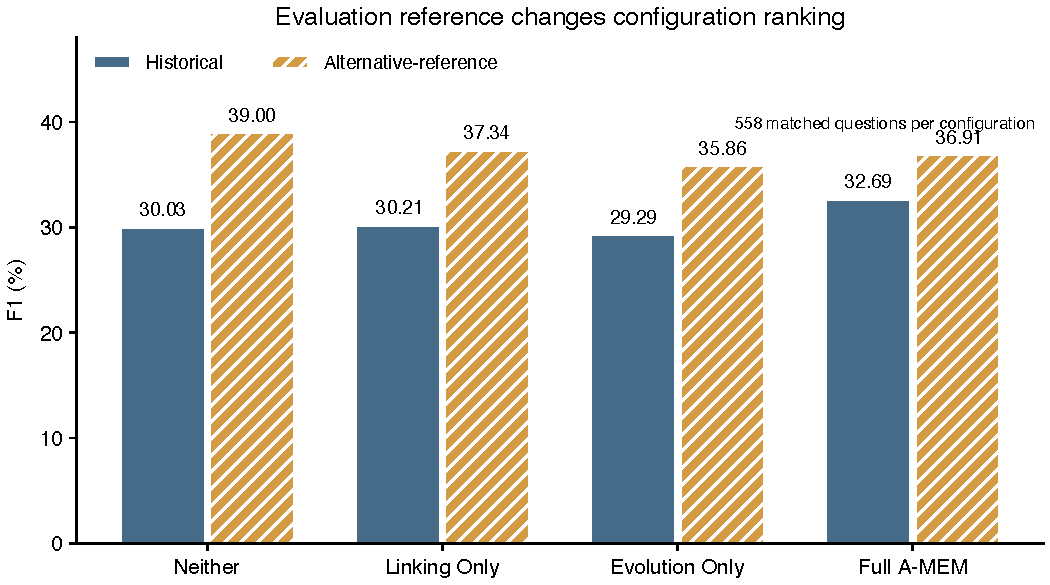
\includegraphics[width=0.93\linewidth]{assets/01_scoring_comparison.pdf}
\caption{Across 558 matched questions per configuration, the historical distractor puts Full first (32.69\% F1). Scoring the same answers against the no-information reference puts Neither first (39.00\%). Only the 121 Category 5 references change.}\label{fig2}
\end{figure}
The paper’s Table~3 reports category scores only. Our supplementary aggregate weights each of the 558 questions equally. Under historical F1, Full led at 32.69\%. Linking Only exceeded Neither by 0.18 points, Full exceeded Linking Only by 2.49, and Evolution Only fell 0.74 below Neither. Under updated author evaluation, Neither led on F1 (39.00\%) and BLEU-1 (35.01\%) and recognised missing information most frequently (86/121). Full abstained appropriately on 71/121.

For each configuration, all 437 questions in Categories~1–4 had identical scores under both policies. The other 121 questions had the same predictions and different references. What surprised me was that changing the reference for those 121 answers was enough to change the aggregate leader, without generating another prediction. To ask what the memory actions contributed, I next compare the independently built configurations under the planned primary metric.

\subsection{Part B: Does neighbour evolution help temporal reasoning?}
\enlargethispage{1.5\baselineskip}
Evolution Only scored 34.17\% temporal F1 against 36.61\% for Neither ($-2.44$ points). With linking enabled, adding evolution raised temporal F1 from 31.62\% to 34.29\% ($+2.67$ points). The $+5.11$-point temporal interaction describes that change in effect. Neither still had the highest absolute temporal F1. Conv-49 differed from the pooled result for evolution alone. On its 33 temporal questions, Evolution Only exceeded Neither by 5.58 points. With one build per cell, conversation differences and stochastic variation cannot be separated.

\begin{table}[H]\centering\small\setlength{\tabcolsep}{4pt}
\begin{tabular*}{\linewidth}{@{\extracolsep{\fill}}lrrr@{}}
\toprule
Population & Evolution Only $-$ Neither & Full $-$ Linking Only & Interaction \\
\midrule
Temporal (89) & $-2.44$ / $-1.53$ & $+2.67$ / $+1.81$ & $+5.11$ / $+3.33$ \\
All questions (558) & $-3.15$ / $-2.72$ & $-0.43$ / $-0.76$ & $+2.72$ / $+1.96$ \\
\bottomrule\end{tabular*}
\caption{Observed evolution contrasts under updated author evaluation. Each pair is the difference in F1/BLEU-1 (percentage points), calculated from unrounded question scores. Interaction subtracts the evolution contrast without linking from the contrast with linking.}\label{tab6}
\end{table}

Across all 558 questions, enabling evolution yielded lower updated F1 both without linking ($-3.15$ points) and with it ($-0.43$). The interaction was $+2.72$ points overall, positive in conv-44 and conv-50 and negative in conv-49. Evolution Only scored below Neither in all three conversations overall and in all five pooled categories. The overall changes from enabling linking were $-1.66$ F1 / $-1.44$ BLEU-1 points without evolution and $+1.06$ / $+0.52$ with evolution.

\begin{figure}[H]\centering
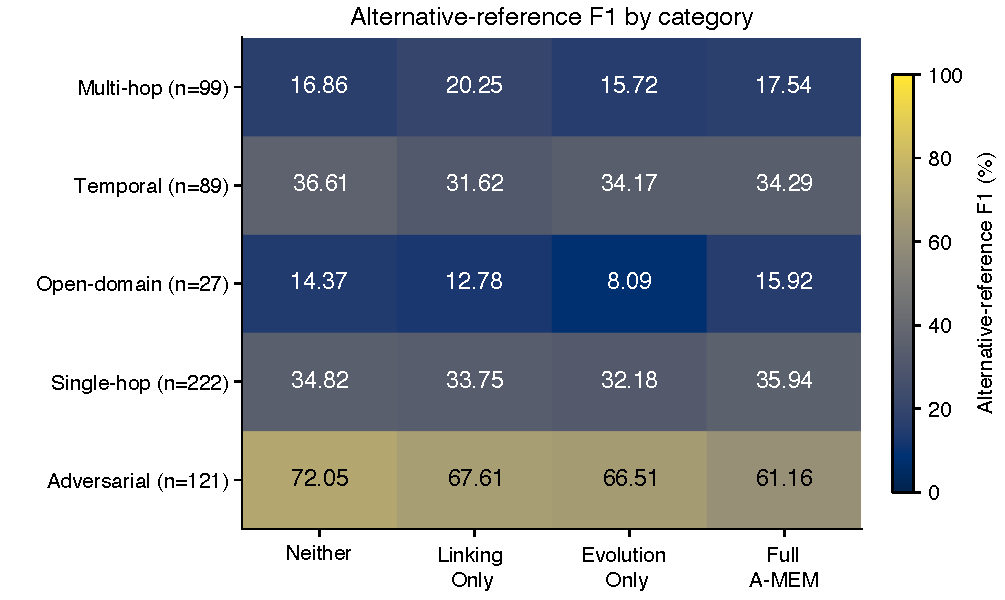
\includegraphics[width=0.92\linewidth]{assets/02_category_heatmap.pdf}
\caption{Updated F1 (\%) on the five categories. The 89 temporal questions address the initial evolution hypothesis. Only the adversarial row changes when the historical reference is used.}\label{fig3}
\end{figure}

Linking Only had the highest multi-hop F1, exceeding Neither by 3.40 points (20.25\% versus 16.86\%, rounded). It also retrieved more entries and used more answer input tokens (Table~\ref{tab7}). These simultaneous differences leave the explanation for the score change open. Full led on open-domain and single-hop F1. The open-domain interaction was large ($+9.41$ points) but rested on just 27 questions. Neither led on updated adversarial F1 (72.05\%), while the historical distractor gave Full the highest adversarial F1 (41.70\%).

\subsection{Quality and model charges across the four configurations}
\enlargethispage{1.5\baselineskip}
Following Professor Nguyen’s Pareto approach, I compare each configuration’s aggregate F1 with its identified model charges. A configuration is dominated if another costs no more and scores at least as well, with a strict advantage on at least one measure.
\begin{table}[H]\centering\small\setlength{\tabcolsep}{4pt}
\begin{tabular}{@{}>{\raggedright\arraybackslash}p{\dimexpr 0.22\linewidth-6.4pt\relax}>{\raggedright\arraybackslash}p{\dimexpr 0.19\linewidth-6.4pt\relax}>{\raggedright\arraybackslash}p{\dimexpr 0.23\linewidth-6.4pt\relax}>{\raggedright\arraybackslash}p{\dimexpr 0.19\linewidth-6.4pt\relax}>{\raggedright\arraybackslash}p{\dimexpr 0.17\linewidth-6.4pt\relax}@{}}
\toprule
Configuration & Retrieved / QA & Answer input tokens & Model USD & Updated F1 \\
\midrule
Neither & 10.00 & 747,640 & \$0.95045 & 39.00 \\
Linking Only & 20.15 & 1,511,478 & \$1.07939 & 37.34 \\
Evolution Only & 10.00 & 749,026 & \$0.95333 & 35.86 \\
Full A-MEM & 19.99 & 1,503,791 & \$1.08084 & 36.91 \\
\bottomrule\end{tabular}
\caption{Matched 558-question scientific inference costs from accepted builds only; excludes failed attempts, held reservations and Langfuse fees.}\label{tab7}
\end{table}
\begin{figure}[H]\centering
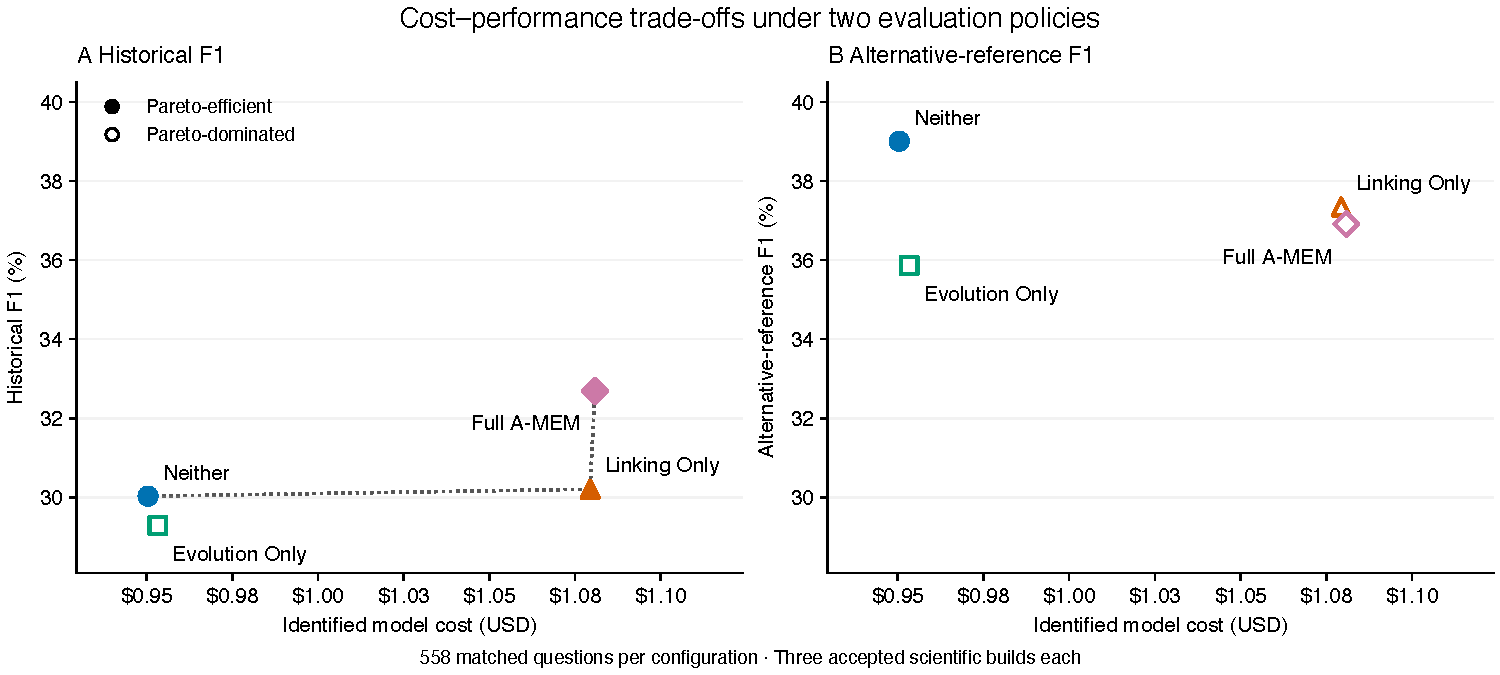
\includegraphics[width=\linewidth]{assets/06_dual_scoring_f1_vs_cost.pdf}
\caption{Cost–performance frontiers under historical and updated F1 (558 matched questions). Historical scores place Neither, Linking Only and Full A-MEM on the observed frontier; updated scores place only Neither on it. Costs include identified model charges from accepted scientific builds, excluding earlier attempts and Langfuse fees.}\label{fig4}
\end{figure}
Across the three accepted builds per configuration, Linking Only increased mean retrieval from 10.00 to 20.15 entries per question and native answer input from 747,640 to 1,511,478 tokens. Its identified model charge rose from \$0.95045 to \$1.07939. Evolution Only incurred just \$0.00288 more than Neither (\$0.95333 versus \$0.95045), with lower aggregate F1 under both policies. Neither therefore dominated Evolution Only on both frontiers. All configurations paid for the shared decision. These realised condition totals include the shared overhead and variation in generated tokens. They do not isolate the price of an individual mutation.

I reconciled identified charges against OpenRouter generation records, checking identities, upstream route, tokens and cost independently against the local ledger. Summed charges also matched wallet and API-key movements. All 1,666 generations in the final clean cell reconciled. The frontier uses only the twelve accepted builds. Failed attempts, held reservations and Langfuse fees appear in the campaign accounting in Section~6.

On the historical frontier, Neither, Linking Only and Full had successively higher charges and observed F1. Under updated F1, Neither alone was Pareto-efficient: it had both the highest aggregate F1 and the lowest identified model cost. The frontier applies to this model, these three conversations and the observed prices.

\section{Debug diary and methodological reflection}
\subsection{The unplanned DeepSeek detour}
I chose DeepSeek because I already had credit and its OpenAI-compatible API appeared to make substitution straightforward. The same request format reached the model, yet structured fields could have unexpected types, JSON could be malformed, and some generations reached their output limit. Transport interruptions also required checkpoint recovery. Handling those cases taught me the limit of API compatibility: it told me how to send a request, but gave me little assurance about the responses the frozen workflow would receive.

Three DeepSeek Flash Full A-MEM lineages completed in Degraded status. Table~\ref{tab8} pools their saved scores by question. On the same 558 questions, DeepSeek had higher observed F1 and BLEU-1 than GPT-4o-mini Full A-MEM under both policies. This comparison was exploratory. Each model contributed one build per conversation, and provider routes, generation caps, compatibility handling and recovery histories differed. Further work on provider compatibility would have taken me further from my question about memory mechanisms. I returned to GPT-4o-mini for the factorial study to keep that comparison close to the authors’ model choice.

\begin{table}[H]\centering\small\setlength{\tabcolsep}{4pt}
\begin{tabular}{@{}>{\raggedright\arraybackslash}p{\dimexpr 0.19\linewidth-6.666666666666667pt\relax}>{\raggedright\arraybackslash}p{\dimexpr 0.09\linewidth-6.666666666666667pt\relax}>{\raggedright\arraybackslash}p{\dimexpr 0.18\linewidth-6.666666666666667pt\relax}>{\raggedright\arraybackslash}p{\dimexpr 0.18\linewidth-6.666666666666667pt\relax}>{\raggedright\arraybackslash}p{\dimexpr 0.18\linewidth-6.666666666666667pt\relax}>{\raggedright\arraybackslash}p{\dimexpr 0.18\linewidth-6.666666666666667pt\relax}@{}}
\toprule
Conversation & QA & Updated F1 & Updated BLEU-1 & Hist. F1 & Hist. BLEU-1 \\
\midrule
conv-44 & 158 & 54.06 & 48.37 & 42.05 & 36.24 \\
conv-49 & 196 & 49.63 & 46.31 & 43.22 & 39.95 \\
conv-50 & 204 & 48.22 & 43.53 & 41.74 & 37.19 \\
Pooled (derived) & 558 & 50.37 & 45.88 & 42.35 & 37.89 \\
\bottomrule\end{tabular}
\caption{Exploratory DeepSeek Flash Full A-MEM results (scores in \%). Three completed Degraded lineages; the pooled row is a derived 558-question aggregate, not part of the primary GPT-4o-mini experiment.}\label{tab8}
\end{table}
\subsection{Provider failures and the final clean run}
The final Linking Only / conv-44 cell exposed a second problem: execution infrastructure could affect the author’s fallback behaviour. The first run disconnected during evolution; the special financial stop escaped the author’s ordinary exception handler, preventing an unevolved note from being inserted. A reviewed recovery completed all 675 memories, but a second disconnect stopped answer generation after 87 of 158 questions. A fresh replacement then stopped on an HTTP 200 response whose generation was marked erroneous. In each case we preserved the failed artifacts rather than silently altering outputs or combining stochastic memory states.

I ultimately chose a final fresh run with broader, predeclared and financially bounded recovery rules while retaining unchanged scientific settings. The successful run completed 675 memories and 158 questions through 1,666 first-transmission model calls, with zero retries. Independent checks reproduced embeddings, retrieval rankings, scores, Langfuse experiment associations and provider charges. The new Linking Only cell was accepted as Clean, and all earlier failures remained available for audit.

Keeping the failed attempts made the final result auditable: I could identify which build supplied each answer and which charges belonged to it. The expensive part in my own time was rechecking the entire financial history after individual failures. For a similar study I would set bounded recovery rules before collection and reconcile new charges as they arrive. That would leave more time to examine the temporal and multi-hop results while preserving the evidence behind them.

There was also an important difference between scientific inference cost and the cost of conducting research. The twelve accepted GPT-4o-mini builds incurred approximately \$4.06 in identified model charges. Campaign-wide identified model charges, including earlier failed attempts and compatibility checks, totalled approximately \$4.70. Broader conservative campaign exposure, including held reservations and a conservative upper bound for Langfuse service, reached \$10.46. Only the accepted-build model charges belong in Section 5’s like-for-like Pareto comparison.

The Clean replacement completed the comparison without reconstructing memories, imputing answers or mixing runs.

\section{Limitations, conclusion and reproducibility evidence}
\subsection{Part A: How much of the published advantage recurs?}
Deterministic Full replay matched the frozen author workflow under the archived responses. Among the three published conditions, Full again won both historical metrics in three of five categories. Only adversarial questions retained the complete ordering. In our supplementary 558-question comparison, Full led historical F1 (32.69\%); changing the reference for 121 questions put Neither first (39.00\%) on identical answers.

\subsection{Part B: What can we attribute to neighbour evolution?}
On temporal questions, updating older notes lowered F1 without linking and raised it with linking ($+5.11$-point interaction). Across all questions both contrasts were negative ($+2.72$ interaction). Neither dominated Evolution Only on cost and aggregate F1 under both policies. Linking Only gained on multi-hop questions while retrieving more entries and using more answer tokens.

\subsection{Limits of inference}
\enlargethispage{1.5\baselineskip}
Table~3’s exact questions and retrieval settings are unverified. I used three of ten conversations, retrieval depth ten and one stochastic build per cell. Conversation differences and run variation cannot be separated; statistical significance remains unestablished. Strengthening jointly changes links and tags, and evolution changes older contexts and tags. Repeated builds, more conversations and separate tests of retrieval depth and individual operations would show how far these findings extend.

This project changed how I read published research. Even after verifying that Full A-MEM matched the frozen implementation in deterministic replay, changing the scoring reference alone changed which configuration performed best on identical predictions. It reinforced for me that published results should not be accepted uncritically: their conclusions depend on the assumptions and evaluation methods behind them. Independent reproduction provides an opportunity to examine those assumptions and establish greater confidence in what the findings actually demonstrate.

\subsection{Sources and development evidence}
Xu et al. (2025), A-MEM: Agentic Memory for LLM Agents, \href{https://arxiv.org/abs/2502.12110v11}{arXiv:2502.12110 (v11)}; original implementation \href{https://github.com/WujiangXu/A-mem/tree/f9a173dec325d84fcc97e7828775c7b241c33466}{WujiangXu/A-mem} (frozen f9a173d); \href{https://snap-research.github.io/locomo/}{LoCoMo benchmark data} distributed with the release. Source, results, commit history and execution instructions are available at \href{https://github.com/alistairkung/A-mem-reproducibility}{github.com/alistairkung/A-mem-reproducibility}.

Accepted twelve-cell scientific evidence: \href{https://github.com/alistairkung/A-mem-reproducibility/commit/8485673183d7b8018c841082d075b21158002700}{8485673183d7b8018c841082d075b21158002700}. The repository archives source and dataset fingerprints, original question IDs, model responses, memory checkpoints and question-level scores. The publication generator pins its scientific inputs to this revision. Reporting assets are in PRs \#53–57; full matched analysis, both scoring policies and independent financial/observability receipts are linked from the repository. The pooled DeepSeek figures in Section 6 are exploratory, not part of the controlled factorial comparison.

\begingroup
\footnotesize\raggedright
\setlength{\parskip}{0pt}
\let\originalthebibliography\thebibliography
\renewcommand{\thebibliography}[1]{\originalthebibliography{#1}\setlength{\itemsep}{2pt}\setlength{\parsep}{0pt}}
\bibliographystyle{unsrturl}
\bibliography{references}
\endgroup
\end{document}
